\chapter{Results}\label{chap:results}
We discussed various scenarios in the previous chapter.
In this chapter, we use them to gauge the quality of our numerical scheme.
We start with a convergence test, followed by three standard testing scenarios.
Next, we simulate two different cloud scenarios and check whether our \amr{} criterion is useful.

\newcommand{\error}{\operatorname{Total-Error}}
\section{Convergence Test}\label{sec:results-convergence}
For the convergence test, we run our manufactured solution scenario~(\cref{sec:manufactured-solution}) for all orders 1 to 6 and for number of cells $3^2, 9^2, 27^2$ and $81^2 $.

Before computing the error we first need to define the $L_p$ norms for a $p > 0$ by
% notation: https://en.wikipedia.org/wiki/Lp_space#Lp_spaces
\begin{equation}
  \label{eq:Lp-nrom}
  \Vert f(x) \Vert_p = \left( \int_K \vert f(x) \vert^p d\mu  \right)^{1/p}.
\end{equation}
We are interested in the total error which we define as the norm of the difference between an analytical solution $f(\bm{x}, t)$ and our approximation $\hat{f}(\bm{x}, t)$.
The error at a time $t$ is thus defined as
\begin{equation}
  \label{eq:error}
  \error(t,p) = \Vert f(\bm{x}, t) - \hat{f}(\bm{x}, t) \Vert_p.
\end{equation}

We first observe that for our approximation space $\broken$ we can split up the error as a sum over all cells.
We evaluate the cell-wise error with Gaussian quadrature using \cref{eq:integration-by-substitution}
 \begin{equation}
%   \Vert f(\bm{x}, t) - \hat{f}(\bm{x}, t) \Vert_p^p =
   \error(t,p) = 
   \left( \sum_{\cell[i] \in \broken}
    \left( V \sum_{\bm{j}} \vert f^{\cell[i]}(\quadNode[j], t) - \hat{f}^{\cell{i}}(\quadNode[j], t) \vert^p \quadWeight[j] \right) \right)^{1/p}.
 \end{equation}
Here, a superscript of $\cell[j]$ denotes the restriction of the function to a grid cell.
To increase the quality of the error computation, we evaluate both analytical and approximate solution at the quadrature nodes of a scheme with 10 quadrature nodes $\quadNode[j]$ with weights $\quadWeight[j]$.
We then use these nodes to compute the approximation error per cell.

For the limiting case of $p \to \infty$ we use the maximum of the point-wise error over all nodal points.

\begin{figure}[htb]
  \centering
  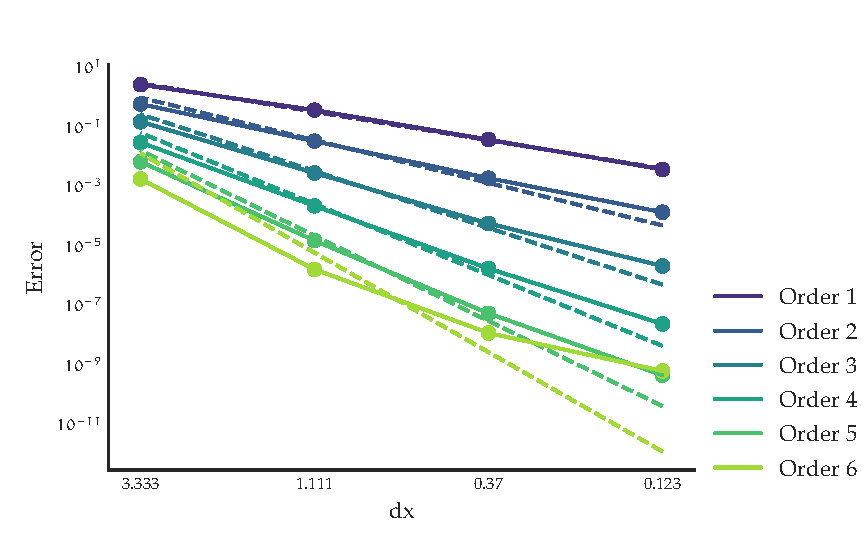
\includegraphics[trim=0.2cm 0.3cm 0.2cm 1.0cm, clip]{thesis_convergence}
  \caption{$L_2$-Error vs.\ Grid Size.
    The dashed lines are the optimal order of convergence $N+1$.
  The line is estimated by a linear regression fit and and setting the slope to the ideal order.}
  \label{fig:convergence-l2-error}
\end{figure}

\begin{table}[htb]
  \centering
\caption{Numerical order of convergence of ADER-DG method}%
\label{tab:convergence-order}
\begin{tabular}{@{}lS[table-format=1.2]S[table-format=1.2]S[table-format=1.2]@{}}
\toprule
{Polynomial Order $N$} & {$L_1$} & {$L_2$} & {$L_\infty$}\\ \midrule
1 & 2.03 & 2.00 & 1.92\\
2 & 2.56 & 2.55 & 2.55\\
3 & 3.43 & 3.40 & 3.44\\
4 & 4.27 & 4.27 & 4.36\\
5 & 5.00 & 5.02 & 5.08\\
6 & 4.46 & 4.50 & 4.65\\
\bottomrule
\end{tabular}
\end{table}

To compute the numerical order of convergence, we perform a linear regression of the logarithm of the error vs.\ the logarithm of the meshsize.
The size of the slope is then the convergence order.
Looking at the plot for the $L_2$ error~(\cref{fig:convergence-l2-error}) shows that our method converges for all tested polynomial orders.
Note that the error for the finest grid with order 6 is worse than the error for order 5.
For all other meshsizes and orders, a higher order indicates a smaller error.
If we compare our errors with the optimal order of convergence, we notice that while order 1 exhibits the theoretical order of convergence of 2, larger polynomial orders lead to diminishing returns.

The same is true for other error norms (\cref{tab:convergence-order}).
This means, that we do not achieve the optimal theoretical order of convergence in general.
In~\cite{dumbser2010arbitrary}, which use a similar numerical method and the same scenario, but a different grid, \citeauthor{dumbser2010arbitrary} achieves the optimal order for most polynomial orders.
Some \textsc{dg}-methods of odd order only achieve a numerical convergence order of $N+\nicefrac{1}{2}$\todo{Odd polynomial order or convergence order?}.

\section{Accurate CFD}\label{sec:cfd}
After we established that our scheme converges, we evaluate it using standard \textsc{cfd} testing scenarios that either have an analytical solution or for which we have a reference solution.
% Show:
% \begin{itemize}
% \item Taylor-Green High Order
%   LIC, Plot v/p ana vs.\ real
% \item ABC Medium Order
%   Plot p ana.\ vs real
% \item Lid-Driven Cavity
%   Show LIC, maybe plot over x?
% \end{itemize}

\sidetitle{Taylor-Green Vortex}
We used an \aderdg{}-scheme of order 5 with a mesh of size $27 \times 27$ cells to simulate the Taylor-Green Vortex.
The simulation ran for \SI{10}{\s}.
Our solution resulted in the expected streamlines (\cref{fig:taylor-green-streamlines}).
Furthermore, we compare our results with the analytical solution for the incrompressible case.
We achieve a small error~(\cref{fig:taylor-green-result}) for both pressure and velocity.
The small errors are expected and not only stem from numerical inaccuracies but primarily from the fact that we simulate a compressible fluid.
Note that the error is small over the entire domain, and not only close to the boundary, where we impose the analytical solution.
Overall, we notice a very good agreement with both the analytical solution and the results of~\cite{dumbser2016high}.

\begin{figure}[htb]
  \centering
  \includegraphics[width=0.5\textwidth]{thesis_taylor_green_stream}
  \caption{Streamlines for Taylor-Green vortex}
  \label{fig:taylor-green-streamlines}
\end{figure}

\begin{figure}[htb]
  \centering
  \begin{subfigure}[t]{0.5\textwidth}
    \centering
    \includegraphics{thesis_taylor_green_vel}
    \caption{Position vs.\ velocity}
  \end{subfigure}~%
  \begin{subfigure}[t]{0.5\textwidth}
    \centering
    \includegraphics{thesis_taylor_green_pressure}
    \caption{Position vs.\ pressure}
  \end{subfigure}
  \caption{\label{fig:taylor-green-result}%
    Comparison of Taylor-Green simulation with analytical solution.
    The former is represented by the scatter plot, the latter by the gray line.
    Note that we only show every 5th point.}
\end{figure}

\sidetitle{ABC Flow}
\begin{figure}[htb]
  \centering
  \includegraphics{thesis_abc_flow_pressure}
  \caption{\label{fig:abc-result}%
  Pressure for the \textsc{abc}-flow.
  Each column represents a one-dimensional slice, all other coordinates are held constant at their median value.
  We compare the analytical solution (gray line) with our approximation (scatter plot).
  We only show every 4th point.}
\end{figure}
We used an \aderdg{}-scheme of order 2 with a mesh consisting of $27 \times 27 \times 27$ cells to simulate the \textsc{abc}-flow.
We ran the simulation for \SI{1}{\s}.
Our solution for the pressure shows an excellent agreement~(\cref{fig:abc-result}) with the analytical solution.
We thus shows that our implementation can also handle three-dimensional scenarios.

\sidetitle{Lid-Driven Cavity}
\begin{figure}[htb]
  \centering
  \begin{subfigure}[t]{0.4\textwidth}
    \centering
    \includegraphics[width=1.2\textwidth]{thesis_lid_driven_cavity_stream}
    \caption{\label{fig:lid-driven-cavity-streamlines}%
      Streamlines of the cavity flow.}
  \end{subfigure}~%
  \begin{subfigure}[t]{0.7\textwidth}
    \centering
    \includegraphics{thesis_lid_driven_cavity}
    \caption{\label{fig:lid-driven-cavity-result}%
      Plot of velocity slices. Lines are our soulution, scatter plot shows reference solution~\cite{ghia1982high}.}
  \end{subfigure}
  
  \caption{Lid-Driven Cavity solution at $t=\SI{30}{\s}$}
  \label{fig:lid-driven-cavity}
\end{figure}
We used a \muscl{}-limited \aderdg{}-scheme of order 3 with a mesh of size $27 \times 27$ for the Lid-Driven Cavity.
The streamlines~(\cref{fig:lid-driven-cavity-streamlines}) agree with the expected solution but have two smaller, secondary vortices in the bottom corners.
They do not appear in the plots of~\cite{dumbser2010arbitrary} but do appear in~\cite{ghia1982high}.
Additionally, we show the velocity along both axes in \cref{fig:lid-driven-cavity-result}.
They too agree with the reference solution of~\cite{ghia1982high}.

Surprisingly, the limiter was not activated at all.
We noticed that we need the limiter when we use a lower speed of sound and thus a flow with larger Mach number.

\section{Accurate Clouds}\label{sec:results-cloud}
We discussed the capabilities of our scheme regarding standard \textsc{cfd} testing scenario.
In this section, we consider our bubble scenarios.
\sidetitle{Cosine Bubble}
\begin{figure}[htb]
  \centering
  \begin{subfigure}[t]{0.5\textwidth}
    \centering
    \includegraphics[scale=1.0]{thesis_cosine_bubble_contour_t700}
    \caption{\label{fig:cosine-bubble-contour-ours}%
      Our result}
  \end{subfigure}~%
  \begin{subfigure}[t]{0.5\textwidth}
    \centering
    \includegraphics{giraldo_results_cosine_bubble}
    \caption{\label{fig:cosine-bubble-contour-giraldo}%
      Figure taken from~\cite{giraldo2008study}, resolution of \SI{20}{\m}, $N = 10$, \dg{}, modified Navier-Stokes} %poly order
  \end{subfigure}
  \caption{\label{fig:cosine-bubble-contour}%
    Contours for the cosine bubble results.
    Contours are $-0.05, -0.025, \ldots 0.525$, excluding zero.
  }
\end{figure}
We ran our first scenario, the cosine bubble, with an \aderdg{}-scheme of order 4 and the adaptive mesh criterion \cref{eq:refinement-criterion} with thresholds of $T_\text{refine} = 2.5$ and $T_\text{delete} = -0.5$.
Our coarsest level has $3^3$ cells, our finest level has $3^4$ cells.
We thus have a resolution of ca.\ \SI{37.037}{\m} up to \SI{12.3457}{\m}.

The coarse structure of our simulation~(\cref{fig:cosine-bubble-contour-ours}) agree with the reference solution~(\cref{fig:cosine-bubble-contour-giraldo} of~\cite{giraldo2008study} but the fine details differ.
In contrast to us, they use a scheme of polynomial order 10 and a uniform spatial resolution of \SI{20}{\m}.
Furthermore, we use a physical viscosity of $0.1$, which explains why we have fewer spurious details while using a lower order.
This becomes more clear, by comparing the potential temperature pertubation.
Our solution has a smooth distribution inside the cloud~(\cref{fig:cosine-bubble-potT-ours}) while the results of~\cite{giraldo2008study} show sharp peaks~(\cref{fig:cosine-bubble-potT-giraldo}).
In addition, our solution does not contain negative values for the pertubation.
Despite the different parameters, the maximum pertubation and its position matches for both results.

\begin{figure}[htb]
  \centering
  \begin{subfigure}[t]{0.5\textwidth}
    \centering
    \includegraphics{thesis_cosine_bubble_pertubation}
    \caption{\label{fig:cosine-bubble-potT-ours}%
      Our result}
  \end{subfigure}~%
  \begin{subfigure}[t]{0.5\textwidth}
    \centering
    \includegraphics{giraldo_results_cosine_bubble_pertubation}
    \caption{\label{fig:cosine-bubble-potT-giraldo}%
      Figure taken from~\cite{giraldo2008study}, resolution of \SI{20}{\m}, $N = 10$, \dg{}3 uses modified Navier-Stokes} %poly order
  \end{subfigure}
  \caption{\label{fig:cosine-bubble-potT}%
    $z$ vs.\ pertubation of potential temperature for the cosine bubble scenario at $t=\SI{700}{\s}$.
  }
\end{figure}


\sidetitle{Two Bubbles}
We ran the second scenario with the same \amr{} settings as the first one.
The results in (\cref{fig:two-bubbles-contour}) are comparable to the reference solution~\cite{muller2010adaptive} for the first seven minutes.
Note that the final plot at \SI{7}{\min} looks different in our simulation.
A possible source for this is that we use a different equation set than~\cite{muller2010adaptive}.
While we use a general purpose set with small modifications for atmospheric flows, they use a equation set that is fully focussed on this scenario.
Furthermore, we use the full Navier-Stokes viscous fluxes instead of an approximation.

% \begin{figure}[p]
%   \vspace*{-4.5cm}
%   \thisfloatpagestyle{empty}
%   \centering
%   \begin{subfigure}{1\textwidth}
%     \centering
%     \includegraphics{thesis_two_bubbles_contour_collage.pdf}
%   \end{subfigure}
%   \vspace*{1cm}
%   \begin{subfigure}[t]{1\textwidth}
%     \centering
%     \includegraphics[trim=0.0cm 0.0cm 0.0cm 0.0cm, clip, scale=1.2]{giraldo_results_two_bubbles}
%   \end{subfigure}
%   \caption{\label{fig:two-bubbles-contour}%
%     Results for two bubble scenario.
%     On the top is our, the bottom plots are taken from~\cite{muller2010adaptive}.
%   Contour values for potential temperature pertubation are $-0.05, 0.05, 0.1, \ldots 0.45$.
% }
% \end{figure}
\begin{figure}[p]
  \thisfloatpagestyle{empty}
  \centering
  \begin{subfigure}[t]{0.5\textwidth}
    \centering
  \includegraphics[trim={0cm 0cm 6cm 0cm},clip]{thesis_two_bubbles_contour_collage_comparison} 
  \caption{Our \amr{} solution.}
  \end{subfigure}~%
  \begin{subfigure}[t]{0.5\textwidth}
    \centering
  % Without z axis on right \includegraphics[trim={8.16cm 0cm 0cm 0cm},clip]{thesis_two_bubbles_contour_collage_comparison} 
  \includegraphics[trim={7.4cm 0cm 0cm 0cm},clip]{thesis_two_bubbles_contour_collage_comparison} 
  \caption{Reference solution from~\cite{muller2010adaptive}.}
  \end{subfigure}
  \caption{\label{fig:two-bubbles-contour}%
     Contours of the potential temperature for two bubble scenario.
     On the left is our solution, the right plots are taken from~\cite{muller2010adaptive}.
     We modified the arrangement of the reference plots and the placement of its axes. 
   Contour values for potential temperature pertubation are $-0.05, 0.05, 0.1, \ldots 0.45$.
  }
\end{figure}

\section{AMR vs Static Mesh}\label{sec:results-tts-amr}
To show the effectiveness of the \amr{} criterion, we compare the two settings:
\begin{description}
\item[AMR] We use a coarse mesh with just $27 \times 27$ cells.
  Each cell can be refined up to three times.
  That is, the cells have sidelengths of roughly $\left(\SI{37.04}{\m}, \SI{12.35}{\m} \right)$.
  As refinement thresholds we use $T_\text{refine} = 2.5$ and $T_\text{delete} = -0.5$ in \cref{eq:refinement-criterion}.
  \todo{Maybe not restate here?}
  They are the exact same settings that we used for the bubble scenarios in the previous section.
\item[Fine] We use a uniform grid where all cells have a sidelength corresponding to the finest mesh of the \amr{}-test case.
  In addition, we disable the reduction of global observables.
\end{description}
Note, that while our \amr{} criterion is able to cope with an additional, coarser level, the current implementation in \exahype{} is unstable for this scenario.
This is why we only report an \amr{} run with one level of dynamic refinement.

\begin{figure}[htb]
  \centering
  \includegraphics{thesis_two_bubbles_contour_t600_noamr} 
  \caption{\label{fig:two-bubbles-noamr-contour}%
    Two bubbles run with fully refined mesh}
\end{figure}
For both settings, we used an \aderdg{}-method of order $4$ and thus have a minimal effective resolution of ca.\ $\SI{3.09}{\m}$.
The final result for the run with the fully refined mesh (\cref{fig:two-bubbles-noamr-contour}) looks identical to the \amr{} results (\cref{fig:two-bubbles-contour}) shown in the previous section.
Note that the \amr{} criterion manages to track the bubble correctly~(\cref{fig:two-bubbles-amr-grid}) and is introduces only small errors~(\cref{fig:two-bubbles-amr-error})\todo{Increase font size a bit more}.

\begin{figure}[htb]
\centering
\begin{subfigure}[t]{0.45\textwidth}
    \centering
    \includegraphics[width=1.0\textwidth]{thesis_two_bubbles_amr_grid} 
    \caption{\label{fig:two-bubbles-amr-grid}%
      Potential temperature of \amr{} solution.}
\end{subfigure}\qquad%
\begin{subfigure}[t]{0.45\textwidth}
    \centering
    \includegraphics[width=1.0\textwidth]{thesis_two_bubbles_amr_error} 
    \caption{\label{fig:two-bubbles-amr-error}%
      Potential temperature of fully refined solution minus \amr{} solution.}
\end{subfigure}

  \caption{%
    \amr{}-grid at $t = \SI{700}{\s}$ for the two bubbles scenario.}
\end{figure}

\sidetitle{Time to solution test}
We now want to compare the time to solution for both settings.
To ensure a fair comparison, we ran both configurations with the same optimisation options:
\begin{verbatim}
"architecture": "hsw",
"shared_memory": 

    "cores": 28,
    "background_job_consumers": 6,
    "properties_file": "sharedmemory.properties",
    "autotuning_strategy": "dummy"
},
"optimisation": {
    "fuse_algorithmic_steps": true,
    "fuse_algorithmic_steps_factor": 0.99,
    "spawn_predictor_as_background_thread": true,
    "spawn_amr_background_threads": true,
    "spawn_update_as_background_thread": true
}
\end{verbatim}
We ran the simulation without plotters to focus on the performance of the numerics and the mesh refinement routines.

We used a single node of the Haswell-nodes of the Supermuc (Phase 2).
The node has two Intel® Haswell Xeon Processor E5-2697 v3 \textsc{cpu}s with 14 cores each.
Both \textsc{cpu}s ran at a frequency of $\SI{1.8}{\GHz}$.

We solely used the \tbb{} parallelisation of \exahype{}.
To find a reasonable parameter for the number of background job consumers, we ran a grid search.
We ran three \amr{} testcases for a simulation time of $\SI{1}{\min}$.
The testcases were identical in setting to the aforementioned \amr{} run, but with two levels of refinement.
The best median performance was achieved by using six background threads.
Note that the results were noisy and it is unclear whether the chosen number of background threads is optimal.

The \amr{}-method took \SI{98654.1}{\s} (\SI{1}{\day} \SI{3}{\hour} \SI{24}{\minute} \SI{14}{\s})
while the fully refined grid took \SI{169071}{\s} (\SI{1}{\day} \SI{22}{\hour} \SI{57}{\minute} \SI{51}{\s}).
In other words, the latter method took over 71\% longer.

To summarise, our \amr{} criterion saved a significant amount of computational effort while preserving the fine details of a fully refined grid.
\section{Reactive Euler \textit{\&} Navier Stokes}\label{sec:results-reactive}
As a final benchmark, we used the reactive Navier-Stokes equations.
We used a limiting \aderdg{}-scheme with an order of 3.
For runs without viscosity we used a meshsize of $81 \times 81$, for the runs with a viscosity of $\mu = 0.01$ we used a coarser mesh consisting in $27 \times 27$ cells.
We chose the smaller grid because our boundary conditions become unstable for finer grids.
A reason for this might be the fact that we are unable to prescribe the gradient at the boundary in the \muscl{} implementation of \exahype{}.
For some runs, we used the \textsc{dmp} settings
\begin{verbatim}
"limiter": {
    "dmp_observables": 3,
    "dmp_relaxation_parameter": 0.05,
    "dmp_difference_scaling": 1e-3,
    "helper_layers": 1
}
\end{verbatim}
where the \texttt{dmp\_relaxation\_parameter} refers to $\varepsilon_0$ and \texttt{dmp\_difference\_scaling} refers to $\varepsilon$ in \cref{eq:limiting-dmp}.
The large value of $\varepsilon_0$ is necessary, as otherwise the full domain is refined.
We use $\Qrho, \pressure$ and $\QZZ$ as \textsc{dmp} variables.
\begin{figure}[tb]
  \centering
  \begin{subfigure}[t]{0.3\textwidth}
    \centering
    \includegraphics{thesis_detonation_euler_nodmp_pressure}
    \caption{Pressure, Euler, no \textsc{dmp}}
  \end{subfigure}~%
  \begin{subfigure}[t]{0.3\textwidth}
    \centering
    \includegraphics{thesis_detonation_euler_dmp_pressure}
    \caption{Pressure, Euler, \textsc{dmp}}
  \end{subfigure}~%
  \begin{subfigure}[t]{0.3\textwidth}
    \centering
    \includegraphics{thesis_detonation_ns_pressure}
    \caption{Pressure, \textsc{NS}, no \textsc{dmp}}
  \end{subfigure}

  \begin{subfigure}[t]{0.3\textwidth}
    \centering
    \includegraphics{thesis_detonation_euler_nodmp_Z}
    \caption{$Z$, Euler, no \textsc{dmp}}
  \end{subfigure}~%
  \begin{subfigure}[t]{0.3\textwidth}
    \centering
    \includegraphics{thesis_detonation_euler_dmp_Z}
    \caption{$Z$, Euler, \textsc{dmp}}
  \end{subfigure}~%
  \begin{subfigure}[t]{0.3\textwidth}
    \centering
    \includegraphics{thesis_detonation_ns_Z}
    \caption{$Z$, \textsc{NS}, no \textsc{dmp}}
  \end{subfigure}
  \caption{\label{fig:detonation-line-plots}%
    Slices along the $x$-axis for our three configurations.
    We only show one half of the slice because the scenario is symmetric.
  }
\end{figure}
The results for runs with and without \textsc{dmp} can be seen in \cref{fig:detonation-line-plots}.
Note, that oscillations appeared for the Euler equations unless we use the \textsc{dmp}-criterion.
This is not the case for the Navier Stokes equations.
This scenario shows the differences between the viscous Navier-Stokes equations and the Euler equations clearly:
The viscous effects smooth out the otherwise sharp curves.

Furthermore, they have the effect that fewer cells are limited~(\cref{fig:detonation-pressure-contour}).
Note that the limiter activation are not symmetric which is unexpected for a radial-symmetric scenario.
The contours for pressure and mass fraction look similar for all considered settings.

It is difficult to compare these results with our references, because they both use different settings.
In constrast to~\cite{helzel2000modified} we use a non-stiff source term and viscous effects,~\cite{hidalgo2011ader} includes viscosity but is limited to one-dimensional scenarios.
Comparing with \cref{fig:detonation-contour-reference} we can see that our simulation captures the overall behaviour of the reaction similar to the stiff simulations of~\cite{helzel2000modified}.
The viscous effects have a similar smoothing effect as in~\cite{hidalgo2011ader}.

\begin{figure}[htb]
  \centering
  \begin{subfigure}[t]{1.0\textwidth}
    \centering
  \includegraphics[trim=0.0cm 2.0cm 0.0cm 2.6cm, clip]{thesis_detonation_contour_pressure_collage} 
  \caption{Contour is $p = 0.5$}
  \end{subfigure}
  \begin{subfigure}[t]{1.0\textwidth}
    \centering
  \includegraphics[trim=0.0cm 2.0cm 0.0cm 2.6cm, clip]{thesis_detonation_contour_Z_collage} 
  \caption{Contour is $Z = 0.5$}
  \end{subfigure}
  \caption{\label{fig:detonation-pressure-contour}%
    Contour plots for the detonation scenario at $t=0.4$.
    From left to right: Euler without \textsc{dmp}, Euler with \textsc{dmp}, Navier Stokes without \textsc{dmp}.
    Red color indicates that a cell is limited.
  }
\end{figure}

\begin{figure}[htb]
    \centering
    \includegraphics[width=0.33\textwidth]{leveque_detonation_mass_fraction}
    \caption{\label{fig:detonation-contour-reference}Reference solution for mass fraction with stiff source.
      Image taken from~\cite{helzel2000modified}.}
\end{figure}


%%% Local Variables:
%%% mode: latex
%%% TeX-master: "../main"
%%% End:
